\documentclass[a4paper,11pt]{article}

\usepackage[utf8]{inputenc}
\usepackage[T2A]{fontenc}
\usepackage[english,russian]{babel}
\usepackage[margin=2.5cm]{geometry}
\usepackage{amsmath,amssymb,amsthm,mathtools}
\usepackage{enumitem}
\usepackage{booktabs}
\usepackage{graphicx}
\usepackage{xcolor}
\usepackage[colorlinks=true,linkcolor=blue,urlcolor=blue,citecolor=blue]{hyperref}
\usepackage{url}
\newcommand{\lean}[1]{\mbox{\path{#1}}}
\emergencystretch=3em

\theoremstyle{plain}
\newtheorem{theorem}{Теорема}[section]
\newtheorem{lemma}[theorem]{Лемма}
\newtheorem{proposition}[theorem]{Утверждение}
\newtheorem{corollary}[theorem]{Следствие}
\theoremstyle{definition}
\newtheorem{definition}[theorem]{Определение}
\theoremstyle{remark}
\newtheorem*{remark}{Замечание}

\newcommand{\R}{\mathbb{R}}
\newcommand{\Q}{\mathbb{Q}}
\newcommand{\abs}[1]{\left\lvert #1 \right\rvert}
\newcommand{\set}[1]{\left\{ #1 \right\}}
\newcommand{\ip}[2]{\langle #1, #2\rangle}
\newcommand{\Rpp}[1][2]{\R^{#1}_{++}}
\newcommand{\Rp}[1][2]{\R^{#1}_{+}}
\DeclareMathOperator{\conv}{conv}
\DeclareMathOperator{\cone}{cone}
\DeclareMathOperator{\Sp}{Sp}
\DeclareMathOperator{\Out}{Out}
\DeclareMathOperator{\Bnd}{Bnd}
\DeclareMathOperator{\interior}{int}
\newcommand{\Sw}{\widehat{\Sp}}
\newcommand{\BOX}{\textup{\textsc{Box}}}
\newcommand{\Cw}{\mathcal C}

\title{Слабая разрешимость в коробке цен при $d=2$ за полиномиальное время}
\author{}
\date{14 октября 2026}

\begin{document}
\maketitle

\begin{abstract}
Цены каждого наблюдения известны с точностью до коробки $Q_{\min}\le Q\le Q_{\max}$. Есть ли в коробке цены, при которых выпуск $y$ слабо разрешим? Доказано, что ответ определяется одной задачей о конусе слабо достижимых множеств для $2T$ углов коробок, а решение, если оно есть, можно взять на диагоналях коробок. При $d=2$ эта задача решается одной задачей о потоке из \path{poly-hardness}, поэтому задача о коробке полиномиальна относительно оракула слабой разрешимости. Ответы «да» и «нет» сертифицируются точно. Критерий проверен в Lean~4. Обсуждается, на что опирается вывод и что можно сделать кроме коробки: области с монотонным путём, профиль отклонений и вопрос о решётке допустимых радиусов. Пример на данных EU KLEMS.
\end{abstract}

\section{Постановка}\label{sec:setup}

Обозначения взяты из заметок (\path{latex/notes.tex}) и из \path{poly-hardness/poly-hardness.tex}. Цены $P=\set{p_t\in\Rpp[d]}_{t\in[T]}$, основной случай $d=2$. Множество $S\subset[T]$ \emph{слабо достижимо}, $S\in\Sw(P)$, если для каждого $t\in S$ существует ненулевой $\xi\in\Rp[d]$ с $\ip{\xi}{p_s-p_t}\ge0$ при всех $s\notin S$. Вектор $y\in\Rp[T]$ \emph{слабо разрешим при $P$}, если $P$ лежит в замыкании множества цен, при которых $y$ неоклассически разрешим.

\textbf{(F1)} Критерий слабой разрешимости из заметок (\lean{NeoTiling.weakSolvable_iff}). При $d\ge2$, $P\ge0$, $y\ge0$ вектор $y$ слабо разрешим при $P$ тогда и только тогда, когда $y\in\cone\set{\mathbf 1_S\mid S\in\Sw(P)}$.

\textbf{Коробка.} Даны рациональные $Q_{\min,t}\le Q_{\max,t}$ из $\Rpp[d]$ и рациональный $y\in\Rp[T]$. Цены $Q=\set{q_t}_{t\in[T]}$ лежат в коробке, $Q\in[Q_{\min},Q_{\max}]$, если
\[
    Q^i_{\min,t}\le q^i_t\le Q^i_{\max,t}\qquad\text{при всех } i\in[d],\ t\in[T].
\]
Границы по каждой цене каждого наблюдения свои, нулевая ширина разрешена. Для краткости $L_t:=Q_{\min,t}$, $U_t:=Q_{\max,t}$. Задача $\BOX(L,U,y)$: существуют ли $Q\in[L,U]$, при которых $y$ слабо разрешим?

\textbf{Углы.} $W:=(L_1,\dots,L_T,U_1,\dots,U_T)$~--- $2T$ точек из $\Rpp[d]$, повторы допустимы. Индексы $t$ и $T+t$ в $W$ обозначим $a_t$ и $b_t$. Положим $\Cw(W):=\cone\set{\mathbf 1_S\mid S\in\Sw(W)}\subset\R^{2T}$.

\textbf{Оракул.} Принадлежность вектора конусу слабо достижимых множеств~--- \emph{оракул слабой разрешимости}. При $d=2$ он реализуется одной задачей о потоке полиномиального размера (F2). Все утверждения о сложности ниже~--- полиномиальность относительно этого оракула.

\section{Входные факты}\label{sec:inputs}

\textbf{(F2)} Теорема о потоке из \path{poly-hardness/poly-hardness.tex} в слабом режиме, в Lean \lean{mem_indicatorCone_iff_flow}. Пусть $P=\set{p_t\in\R^2}_{t\in[T]}$ произвольно, положительность, различие точек и общее положение не предполагаются. Тогда $y\in\cone\set{\mathbf 1_S\mid S\in\Sw(P)}$ в том и только в том случае, когда существуют поток $f$ из $\sigma$ в $\tau$ в графе цепочек $G_P$ и вектор $g$ с
\[
    y=\sum_ef_e\mathbf 1_{\Out_e}+g,\qquad 0\le g\le\sum_ef_e\mathbf 1_{\Bnd_e}.
\]
В графе $O(T^2)$ вершин и $O(T^3)$ дуг. Задача о столбце $\max\set{\lambda(S)\mid S\in\Sw(P)}$~--- длиннейший путь в $G_P$.

\textbf{(F3)} Лемма о кубе (\lean{PolyHardness.cube_mem_span}). Если $R_{\min}\subset R_{\max}$ и $\mathbf 1_{R_{\min}}\le v\le\mathbf 1_{R_{\max}}$, то $v$~--- выпуклая комбинация индикаторов $\mathbf 1_R$ с $R_{\min}\subset R\subset R_{\max}$.

\begin{lemma}[достижимость и внутренность]\label{lem:interior}
    Пусть $V\subset\R^d$~--- конечное множество с индексами $I$, $S\subset I$ и $K:=\conv\set{V_r\mid r\notin S}+\Rp[d]$ ($K=\varnothing$ при $S=I$).
    \begin{enumerate}[label=(\alph*)]
        \item Для любой точки $v\in\R^d$: $v\notin\interior K$ тогда и только тогда, когда существует ненулевой $\xi\ge0$ с $\ip{\xi}{z-v}\ge0$ при всех $z\in K$. Если $v\notin K$, то существует ненулевой $\xi\ge0$ с $\ip{\xi}{z}>\ip{\xi}{v}$ при всех $z\in K$.
        \item $S$ слабо достижимо тогда и только тогда, когда ни одна точка $V_t$, $t\in S$, не лежит в $\interior K$.
    \end{enumerate}
\end{lemma}

\begin{proof}
    $K$~--- замкнутое выпуклое множество с $K+\Rp[d]\subset K$. Поэтому $\interior K+\Rp[d]\subset\interior K$.

    (a) Если $\xi$ подходит для $v$, то $K$ лежит в полупространстве $\set{\ip{\xi}{z}\ge\ip{\xi}{v}}$, внутренность которого не содержит $v$. Обратно, пусть $v\notin\interior K$. Отделимость открытого выпуклого $\interior K$ от $v$ даёт $\xi\ne0$ с $\ip{\xi}{z}\ge\ip{\xi}{v}$ на $\interior K$, а значит и на $K=\overline{\interior K}$. Если бы $\xi^i<0$, то $\ip{\xi}{z}$ было бы неограничено снизу вдоль направления $e_i$. Значит, $\xi\ge0$. Для $v\notin K$ берём строгое разделение.

    (b) Это (a) для $v=V_t$: точки $V$ вне $S$~--- образующие $K$.
\end{proof}

Часть (a) нужна для углов $L_t$, $U_t$, которые не обязаны быть точками исходной конфигурации.

\begin{lemma}[выход вдоль монотонного пути]\label{lem:exit}
    Пусть $K\ne\varnothing$ как выше и $z\colon[0,1]\to\R^d$ непрерывно и покоординатно не убывает. Тогда $\set{s\mid z(s)\notin\interior K}$~--- пустое множество или замкнутый отрезок $[0,\ell]$, а $\set{s\mid z(s)\notin K}$~--- пустое множество или полуинтервал $[0,\ell')$ или $[0,1]$.
\end{lemma}

\begin{proof}
    $K$ замкнуто, $\interior K$ открыто, оба переходят в себя при прибавлении векторов из $\Rp[d]$, а $z$ непрерывен и не убывает.
\end{proof}

\section{Точный критерий}\label{sec:thm1}

\begin{theorem}[критерий для коробки]\label{thm:box}
    Пусть $d\ge2$, $L_t\in\Rpp[d]$, $L_t\le U_t$ при всех $t$ и $y\ge0$. Тогда $\BOX(L,U,y)$ выполнено в том и только в том случае, когда существует $w\in\Cw(W)$ с $w(a_t)\ge y_t\ge w(b_t)$ при всех $t$.
\end{theorem}

\begin{proof}
    ($\Rightarrow$) Пусть $L_t\le q_t\le U_t$ и $y$ слабо разрешим при $Q$. По (F1) $y=\sum_k\lambda_k\mathbf 1_{S_k}$, $\lambda_k>0$, $S_k\in\Sw(Q)$. Положим $K_k:=\conv\set{q_r\mid r\notin S_k}+\Rp[d]$. По лемме~\ref{lem:interior} $q_t\notin\interior K_k$ при $t\in S_k$. Определим множество $S'_k$ индексов $W$: $a_t\in S'_k$, если $L_t\notin\interior K_k$, и $b_t\in S'_k$, если $U_t\notin K_k$.

    \emph{$S'_k$ слабо достижимо при $W$.} Каждая точка $W$ вне $S'_k$~--- это $L_r\in\interior K_k$ или $U_r\in K_k$, то есть лежит в $K_k$. Для $v\in S'_k$ лемма~\ref{lem:interior}(a) даёт ненулевой $\xi\ge0$ с $\ip{\xi}{z-v}\ge0$ на $K_k$, в частности на точках $W$ вне $S'_k$.

    Положим $w:=\sum_k\lambda_k\mathbf 1_{S'_k}\in\Cw(W)$. Если $t\in S_k$, то $q_t\notin\interior K_k$ и $L_t\le q_t$, поэтому $L_t\notin\interior K_k$ и $a_t\in S'_k$. Значит, $w(a_t)\ge y_t$. Если $t\notin S_k$, то $q_t\in K_k$ и $U_t\ge q_t$, поэтому $U_t\in K_k$ и $b_t\notin S'_k$. Значит, $w(b_t)\le y_t$.

    ($\Leftarrow$) Пусть $w=\sum_km_k\mathbf 1_{S_k}$, $m_k>0$, $S_k\in\Sw(W)$ и $w(a_t)\ge y_t\ge w(b_t)$. Положим $K_k:=\conv\set{W_u\mid u\notin S_k}+\Rp[d]$. По лемме~\ref{lem:interior} из $a_t\in S_k$ следует $L_t\notin\interior K_k$, а из $b_t\notin S_k$ следует $U_t\in K_k$.

    Для каждого $t$ возьмём диагональ $z_t(s)=L_t+s(U_t-L_t)$, $s\in[0,1]$, и функции
    \[
        \mathrm{hi}_t(s)=\sum_km_k\mathbf 1[z_t(s)\notin\interior K_k],\qquad
        \mathrm{lo}_t(s)=\sum_km_k\mathbf 1[z_t(s)\notin K_k],
    \]
    где пустое $K_k$ даёт вклад $m_k$ в обе. По лемме~\ref{lem:exit} $\mathrm{hi}_t$ не возрастает и полунепрерывна сверху, $\mathrm{lo}_t$ не возрастает и полунепрерывна снизу, $\mathrm{lo}_t\le\mathrm{hi}_t$. На концах $\mathrm{hi}_t(0)\ge w(a_t)\ge y_t$ и $\mathrm{lo}_t(1)\le w(b_t)\le y_t$.

    Положим $s^*_t:=\max\set{s\in[0,1]\mid\mathrm{hi}_t(s)\ge y_t}$. Максимум достигается по полунепрерывности сверху. Если $s^*_t<1$, то $\mathrm{lo}_t\le\mathrm{hi}_t<y_t$ на $(s^*_t,1]$, и полунепрерывность снизу даёт $\mathrm{lo}_t(s^*_t)\le y_t$. Итак, $\mathrm{lo}_t(s^*_t)\le y_t\le\mathrm{hi}_t(s^*_t)$.

    Положим $q_t:=z_t(s^*_t)$, $R_{\min,k}:=\set{t\mid q_t\notin K_k}$ и $R_{\max,k}:=\set{t\mid q_t\notin\interior K_k}$. Тогда $\sum_km_k\mathbf 1_{R_{\min,k}}\le y\le\sum_km_k\mathbf 1_{R_{\max,k}}$. Любое $R$ с $R_{\min,k}\subset R\subset R_{\max,k}$ слабо достижимо при $Q$: для $t\in R$ лемма~\ref{lem:interior}(a) даёт $\xi\ge0$ с $\ip{\xi}{z-q_t}\ge0$ на $K_k$, а каждое $r\notin R$ лежит вне $R_{\min,k}$, то есть $q_r\in K_k$. Запишем $y=\sum_km_kv_k$ с $\mathbf 1_{R_{\min,k}}\le v_k\le\mathbf 1_{R_{\max,k}}$. По (F3) каждый $v_k$~--- выпуклая комбинация индикаторов таких $R$. Значит, $y\in\cone\set{\mathbf 1_S\mid S\in\Sw(Q)}$, и по (F1) $y$ слабо разрешим при $Q$.
\end{proof}

\begin{corollary}[диагональ]\label{cor:diag}
    Если в коробке есть цены, при которых $y$ слабо разрешим, то такие цены есть и на диагоналях: $q_t=L_t+s_t(U_t-L_t)$ со своим $s_t\in[0,1]$ для каждого $t$.
\end{corollary}

\begin{proof}
    По ($\Rightarrow$) существует $w$, и построение ($\Leftarrow$) кладёт $q_t$ на диагональ.
\end{proof}

Смысл следствия. Важно лишь, достаточно ли точка низко-слева, чтобы её можно было отделить от остальных, и достаточно ли высоко-справа, чтобы попасть в оболочку остальных. Оба свойства монотонны, поэтому хватает одного параметра на наблюдение, а сдвиги поперёк диагонали ничего не дают. Если коробка в логарифмах симметрична и одинакова по координатам, $[p_te^{-r},p_te^{r}]$, то диагональ пропорциональна $p_t$, и решение лишь масштабирует цены наблюдения. Если допуски по координатам разные, диагональ меняет и относительные цены, но только в заданную коробкой сторону.

Общее положение, увеличение коробки и компактность не нужны. Размерность входит только через (F1), поэтому теорема и следствие верны при любом $d\ge2$.

\section{Алгоритм и полиномиальность}\label{sec:alg}

\begin{theorem}[алгоритм]\label{thm:alg}
    При $d=2$ условие теоремы~\ref{thm:box}~--- линейная задача допустимости с $O(T^3)$ переменными, $O(T^2)$ строками и коэффициентами $0,\pm1$. Задача $\BOX(L,U,y)$ решается за время, полиномиальное от $T$ и длины записи $(L,U,y)$.
\end{theorem}

\begin{proof}
    Граф цепочек $G_W$ строится по $2T$ углам точными сравнениями координат и знаками $\chi$ для $O(T^3)$ троек. Числа $\chi$ от трёх входных точек имеют полиномиальную длину. По теореме~\ref{thm:box} и (F2) $\BOX$ равносильно допустимости системы: $f\ge0$ на дугах, сохранение потока во внутренних вершинах, $0\le g_q\le\sum_{e:\,q\in\Bnd e}f_e$ и
    \[
        \sum_{e:\,a_t\in\Out e}f_e+g_{a_t}\ge y_t,\qquad
        \sum_{e:\,b_t\in\Out e}f_e+g_{b_t}\le y_t\qquad(t\in[T]).
    \]
    Допустимость рациональной задачи ЛП проверяется за полиномиальное время методом эллипсоидов или внутренних точек.
\end{proof}

\begin{theorem}[свидетель]\label{thm:witness}
    Если $\BOX(L,U,y)$ выполнено, по решению задачи ЛП за полиномиальное время строятся рациональные $Q\in[L,U]$ на диагоналях и точный сертификат: рациональные $m_k\ge0$ и слабо достижимые при $Q$ множества $S_k$ с $\sum_km_k\mathbf 1_{S_k}=y$.
\end{theorem}

\begin{proof}
    \emph{Множества при $W$.} Поток раскладывается на пути. Для пути $\pi$ каждое множество $\Out(\pi)\cup B'$, $B'\subset\Bnd(\pi)$, слабо достижимо при $W$. В Lean это \lean{flow_decomposition} и \lean{isReachableB_iff_path}. Положим $\varphi_q:=g_q/\sum_ef_e[q\in\Bnd e]\in[0,1]$. Вклад пути $\mathbf 1_{\Out(\pi)}+\sum_{q\in\Bnd(\pi)}\varphi_q\mathbf 1_q$ раскладывается по множествам уровня $\varphi$, которые образуют цепь. Так $w=\sum_km_k\mathbf 1_{S_k}$ с $S_k\in\Sw(W)$.

    \emph{Точка $Q$.} Область $K_k=\conv(W\setminus S_k)+\Rp[2]$ задаётся неравенствами $\ip{\xi_j}{z}\ge c_j$ с рациональными $\xi_j\ge0$: нормали рёбер оболочки и $(1,0)$, $(0,1)$. Поэтому выход диагонали из $\interior K_k$ происходит в рациональной точке
    \[
        \lambda_k=\min\Bigl(1,\ \max_j\frac{c_j-\ip{\xi_j}{L_t}}{\ip{\xi_j}{U_t-L_t}}\Bigr),
    \]
    и $\mathrm{hi}_t(s)=\sum_km_k\mathbf 1[s\le\lambda_k]$. Значит, $s^*_t$ из доказательства теоремы~\ref{thm:box} равно одному из $\lambda_k$ (или $1$ при $y_t=0$), и $Q$ рационально.

    \emph{Сертификат при $Q$.} Для $\theta_t:=(y_t-\mathrm{lo}_t(s^*_t))/(\mathrm{hi}_t(s^*_t)-\mathrm{lo}_t(s^*_t))$ множества уровня $\theta$ на $R_{\max,k}\setminus R_{\min,k}$ образуют цепь между $R_{\min,k}$ и $R_{\max,k}$. Они слабо достижимы при $Q$ по доказательству теоремы~\ref{thm:box}, и их массы дают $y$.
\end{proof}

\begin{proposition}[сертификат отказа]\label{prop:refute}
    Пусть $\lambda\in\Q^{2T}$, $\lambda_{a_t}\le0\le\lambda_{b_t}$ при всех $t$, $\sum_t(\lambda_{a_t}+\lambda_{b_t})y_t<0$ и $\lambda(S)\ge0$ для каждого $S\in\Sw(W)$. Тогда $\BOX(L,U,y)$ не выполнено. Если задача ЛП теоремы~\ref{thm:alg} неразрешима, такой $\lambda$ существует. Условие $\lambda(S)\ge0$ на $\Sw(W)$ проверяется одной задачей о столбце: длиннейшим путём в $G_W$ с весами $-\lambda$.
\end{proposition}

\begin{proof}
    Пусть $w\in\Cw(W)$ и $w(a_t)\ge y_t\ge w(b_t)$. Тогда $\ip{\lambda}{w}\ge0$, так как $w$~--- неотрицательная комбинация индикаторов с $\lambda(S)\ge0$. С другой стороны, $\lambda_{a_t}w(a_t)\le\lambda_{a_t}y_t$ и $\lambda_{b_t}w(b_t)\le\lambda_{b_t}y_t$, откуда $\ip{\lambda}{w}<0$. Противоречие. Обратное~--- лемма Фаркаша для конечно порождённого конуса $\Cw(W)$.
\end{proof}

\begin{remark}[о реализации]
    Код решает задачу ЛП методом внутренней точки. Симплекс-метод не используется. Ответ «да» затем проверяется точно в рациональной арифметике по теореме~\ref{thm:witness}: каждое множество сертификата проверяется определением достижимости. Ответ «нет» проверяется по утверждению~\ref{prop:refute}: вектор $\lambda$ берётся из двойственного решения, округляется до рационального и проверяется одним вызовом задачи о столбце из \path{poly-hardness}.
\end{remark}

\section{За пределами коробки}\label{sec:beyond}

\subsection{На что опирается вывод}

Доказательство теоремы~\ref{thm:box} использует пять свойств.
\begin{enumerate}[label=(\roman*)]
    \item Критерий (F1). Слабая разрешимость определена через замыкание, поэтому ответ точный, без зазора между строгой и нестрогой постановкой.
    \item Монотонность. Нормали $\xi$ неотрицательны, поэтому условия «$z\notin\interior K$» и «$z\notin K$» сохраняются при сдвиге $z$ вниз. Нижний угол коробки~--- лучшая точка, чтобы войти в слабо достижимое множество, верхний~--- лучшая, чтобы остаться вне него.
    \item Полунепрерывность. Условие «$z\notin\interior K$» замкнуто, «$z\notin K$» открыто. Вдоль непрерывного монотонного пути это даёт точку $s^*_t$.
    \item Лемма о кубе (F3).
    \item Наблюдения независимы: ограничение имеет вид $q_t\in R_t$ отдельно для каждого $t$.
\end{enumerate}
Полиномиальность опирается только на оракул (F2) при $d=2$, вызванный на $2T$ углах. От коробки используется лишь следующее: $R_t$ лежит между $L_t$ и $U_t$, содержит оба угла и непрерывный монотонный путь между ними. Коробка~--- простейшее такое множество, но не единственное.

\subsection{Области с монотонным путём}

\begin{proposition}[монотонный путь]\label{prop:path}
    Пусть для каждого $t$ задано $R_t\subset\Rpp[d]$, покоординатные $L_t:=\inf R_t$ и $U_t:=\sup R_t$ лежат в $R_t$, и в $R_t$ есть непрерывный покоординатно неубывающий путь из $L_t$ в $U_t$. Тогда цены $q_t\in R_t$ со слабо разрешимым $y$ существуют в том и только в том случае, когда выполнено $\BOX(L,U,y)$.
\end{proposition}

\begin{proof}
    Необходимость: $R_t\subset[L_t,U_t]$. Достаточность: доказательство теоремы~\ref{thm:box}, в котором диагональ заменена путём. Лемма~\ref{lem:exit} верна для любого такого пути. Построенная точка $q_t$ лежит на пути, то есть в $R_t$.
\end{proof}

Утверждение~\ref{prop:path} доказано только в тексте. В Lean проверен случай отрезка: лемма \lean{exists_point_between}.

Примеры.
\begin{enumerate}[label=(\alph*)]
    \item \emph{Коробка с ограничением на относительную цену}: $R_t=\set{q\in[L_t,U_t]\mid c_t\le q^1/q^2\le C_t}$ при $L_t,U_t\in R_t$. Вдоль диагонали $q^1/q^2$ монотонно, поэтому диагональ лежит в $R_t$, и ограничение ничего не меняет.
    \item \emph{Шар} в логарифмах цен углов описанной коробки не содержит. Для него есть только оценки: если $\BOX$ выполнено для вписанной коробки (радиус $\rho/\sqrt d$ по каждой координате), то решение есть и в шаре радиуса $\rho$, а если $\BOX$ не выполнено для описанной коробки, то его нет. Точный критерий для шаров не получен.
\end{enumerate}

\subsection{Профиль отклонений и решётка радиусов}\label{sec:profile}

Для цен $Q$ отклонение каждой из $2T$ цен равно $\delta^i_t=\abs{\ln q^i_t-\ln p^i_t}$. Пусть $\mathcal R$~--- множество векторов радиусов $r=(r^i_t)$, для которых существуют $Q$ с $\delta^i_t\le r^i_t$ и слабо разрешимым $y$. Каждая проверка $r\in\mathcal R$~--- один вызов $\BOX$ с коробкой $[p^i_te^{-r^i_t},p^i_te^{r^i_t}]$. Множество $\mathcal R$ замкнуто вверх и замкнуто.

\textbf{Максимум.} Наименьший общий радиус $\min\set{\rho\mid(\rho,\dots,\rho)\in\mathcal R}$ находится двоичным поиском, $O(\log(1/\varepsilon))$ вызовов оракула.

\textbf{Профиль}~--- лексикографический минимум убывающей перестановки вектора $(r^i_t)$ по $r\in\mathcal R$, как в нуклеолусе. Стадия: найти наименьший общий радиус $\rho$ свободных цен при уже зафиксированных остальных, затем по очереди пытаться опустить каждую свободную цену ниже $\rho$, сохраняя уже опущенные. Цена, которую опустить нельзя, фиксируется на $\rho$. Раз $\rho$ наименьший, хотя бы одна такая цена найдётся. Стадий не больше $2T$, на каждой полиномиальное число вызовов.

\textbf{Решётка.} Открытый вопрос: замкнуто ли $\mathcal R$ относительно покоординатного минимума? Иначе: если две коробки с общими центрами $p_t$ обе содержат решение, содержит ли решение их пересечение? Если да, то $\mathcal R$~--- решётка с наименьшим элементом $r_{\min}$. Тогда профиль~--- это отсортированный $r_{\min}$, он не зависит от порядка проверки, и вся процедура точна и полиномиальна. Если нет, результат стадий может зависеть от порядка проверки, и точность профиля после первой стадии не доказана. Множество цен, при которых $y$ слабо разрешим, вообще невыпукло, поэтому ответ не очевиден.

\subsection{Размерность}

Теорема~\ref{thm:box} верна при любом $d\ge2$, но при $d=3$ уже проверка слабой разрешимости при фиксированных ценах NP-полна (\path{np-hardness}). Это частный случай $L=U$. Поэтому полиномиальность получена только при $d=2$.

\section{Пример}\label{sec:example}

\textbf{Данные.} EU KLEMS 2023, США, вся экономика, 1995--2020, $T=26$ (\path{data/us_tot.csv}). Цены $p_t=(p^K_t/p^{II}_t,\ p^L_t/p^{II}_t)$ после деления каждой исходной цены на её максимум по годам. Выпуск $y_t$~--- объём валового выпуска.

\textbf{Задача.} Найти наименьший максимум логарифмических отклонений $\max_{i,t}\abs{\ln q^i_t-\ln p^i_t}$ по всем $2T$ ценам, при котором $y$ слабо разрешим. Это наименьшее $\rho$, при котором выполнено $\BOX$ для коробки $Q^i_{\min,t}=p^i_te^{-\rho}$, $Q^i_{\max,t}=p^i_te^{\rho}$. Оно находится делением отрезка пополам, на каждом шаге один вызов оракула.

\textbf{Результат.} При наблюдаемых ценах $y$ не слабо разрешим. Наименьший максимум отклонений $\rho^*\approx0{,}0897$, то есть $\pm9{,}4\%$. Оба конца проверены точно. При $\rho^*(1-10^{-4})$ ответ «нет» сертифицирован рациональным вектором Фаркаша (утверждение~\ref{prop:refute}). При $\rho^*(1+10^{-4})$ построены рациональные цены в коробке и сертификат из $48$ слабо достижимых множеств (теорема~\ref{thm:witness}).

\begin{figure}[ht]
\centering
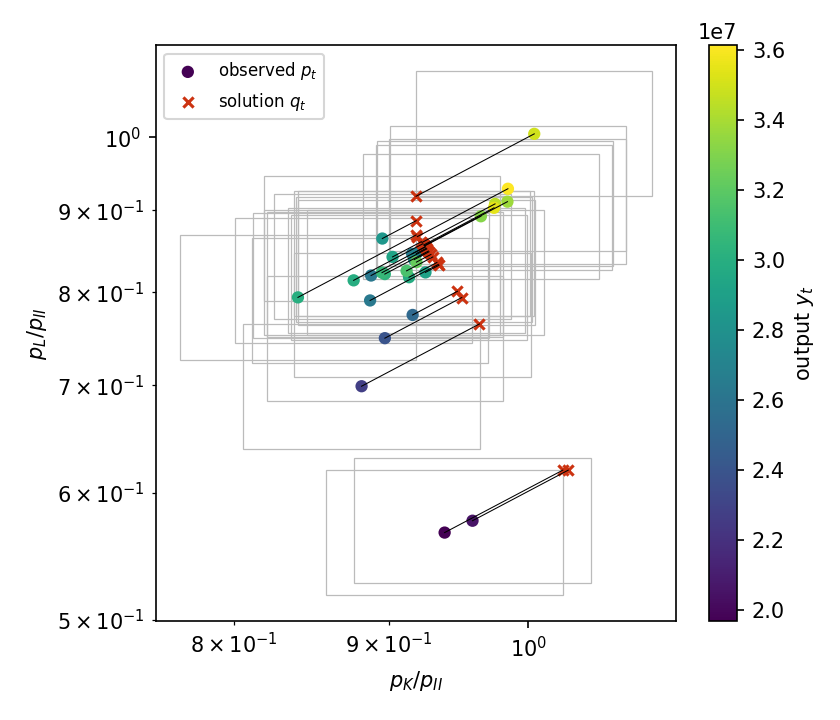
\includegraphics[width=0.6\textwidth]{example.png}
\caption{Нормированные цены, коробки при $\rho=\rho^*(1+10^{-4})$, наблюдения $p_t$ (цвет~--- $y_t$) и решение $q_t$ (крестики). Оси логарифмические.}
\end{figure}

\section{Вычисления}\label{sec:code}

Код лежит в \path{box-perturbation/}: \path{box.py} (задача ЛП, свидетель, сертификаты, использует \path{poly-hardness/planar.py}), \path{example.py} (раздел~\ref{sec:example}), тесты \path{tests/test_box.py}. Тесты сравнивают ответ с определением на малых примерах: перебор $2^T$ множеств и сетка $\set{L,\tfrac{L+U}2,U}^2$ в каждой коробке, вырожденные коробки (нулевые ширины, совпадающие и коллинеарные углы), случай $L=U$. Каждый свидетель проверяется точно, ответы «нет» сертифицируются по утверждению~\ref{prop:refute}.

\section{Проверка в Lean}\label{sec:lean}

Файлы \path{box-perturbation/lean/BoxPerturbation/Support.lean} и \path{Box.lean} (импортируют \path{NeoTiling.Closure} и \path{PolyHardness.FlowLP}). Проверка: \texttt{lake build BoxPerturbation} из корня проекта. Нет \lean{sorry}, аксиомы только стандартные (\lean{propext}, \lean{Classical.choice}, \lean{Quot.sound}).

Теорема~\ref{thm:box}~--- \lean{box_iff}. Слабая разрешимость в формулировке~--- определение через замыкание (\lean{WeakSolvable}), а правая часть~--- обращение к оракулу: принадлежность конусу слабо достижимых множеств углов \lean{Fin.append L U}. Выпуклые оболочки заменены предикатами \lean{Supported} ($z\notin\interior K$) и \lean{StrictlySupported} ($z\notin K$).
\begin{center}
\begin{tabular}{@{}ll@{}}
\toprule
Утверждение & Lean \\
\midrule
Лемма~\ref{lem:interior} & \lean{isWeakReachable_of_supported} \\
Лемма~\ref{lem:exit} & \lean{isClosed_setOf_supported}, \lean{isOpen_setOf_strictlySupported} \\
Точка $s^*_t$ & \lean{exists_mem_Icc_between}, \lean{exists_point_between} \\
(F3) для сумм & \lean{mem_indicatorCone_of_ind_le}, \lean{mem_indicatorCone_of_between} \\
Множества $S'_k$ & \lean{exists_corner_set} \\
Теорема~\ref{thm:box} & \lean{box_iff} \\
\bottomrule
\end{tabular}
\end{center}
Не формализованы: полиномиальность как утверждение о сложности (в Mathlib нет классов сложности), следствие~\ref{cor:diag} отдельной теоремой (в Lean оно содержится в доказательстве \lean{box_iff}), теорема~\ref{thm:witness}, утверждения~\ref{prop:refute} и~\ref{prop:path}, раздел~\ref{sec:profile}.

\end{document}
